\documentclass[a4paper,11pt]{report}
\usepackage[utf8x]{inputenc}
\usepackage{amsmath}
\usepackage{graphicx,color}           % Packages for graphics and color
\usepackage[left=1.5in, right=1in, top=1in, bottom=1in, includefoot, headheight=13.6pt]{geometry}
\usepackage[T1]{fontenc}               % Ensure correct font encoding
\usepackage{hyperref}
\usepackage{algorithmic}
\usepackage{algorithm}
\usepackage{verbatim}
\usepackage{tikz}

\setcounter{secnumdepth}{-1} 
\renewcommand{\chaptername}{}
\renewcommand{\thechapter}{}
\renewcommand{\thesection}{}
\renewcommand{\thesubsection}{}

\begin{document}
\title{
\huge{\textbf{Training Neural Networks for Classification using a Gene Expression Programming Framework}}\\[1.4cm]
\large{by}\\[0.2cm]
\large{Morley Abbott, 100744273} \\[1.4cm]
\large{Supervised by Dr. Anthony White} \\[0.2cm]
\large{School of Computer Science}\\[1.4cm]
\large{Honours Project (COMP 4905)} \\[0.2cm]
\large{Submitted in partial fullfilment of the} \\[0.2cm]
\large{requirements for the degree of } \\[0.2cm]
\large{Bachelor of Computer Science} \\[1.4cm]
\large{at}\\[1.4cm]
\large{Carleton University} \\[0.2cm]
\large{Ottawa, Ontario, Canada} \\[0.2cm]
\large{April, 2011} \\[0.2cm]}
\author{} \date{}

\maketitle


\chapter*{Abstract}

Classification is a major part of machine learning, and is used everyday on large scales:
Google identifies different types of searches and users; Amazon identifies
what kind of people will like a given book; medical clinics can quickly and accurately 
give a diagnosis for a list of symptoms. The basic pattern of converting an input vector 
of data into one item from a set of possible classes is used in applications everywhere. 
Much research is done towards finding more powerful tools to accurately build these classification 
systems.

Evolutionary Computing a powerful and useful tool in many application 
areas in which the search space of potential solutions is very large, and good solutions
can relate to one another. By implementing nature's evolution algorithms in our own ways, we can quickly 
find partial solutions, and combine them into better solutions. This simple process can be 
used in a variety of applications. One such area is artificial neural networks, used to model complex
relationships between inputs and outputs, and discover patterns in data.

This paper utilizes a specific type of evolutionary algorithm, Gene Expression Programming,
and uses it to create artificial neural networks for classification. To do this, a highly expandable 
framework for using Gene Expression Programming is presented, along with some results of tests done 
with it. The paper will begin with a description of the Gene Expression Programming algorithm, and 
how it can be used to create artificial neural networks. This will be followed by an explanation 
of the framework developed, how it works, and some experiments done using the framework. Finally,
the results of the tests will be presented, along with some conclusions, a description of the 
concepts learned, and a short discussion on potential future work with the framework. 


\addcontentsline{toc}{chapter}{Acknowledgements}
\chapter*{Acknowledgements}
I would like to thank Dr. Anthony White for having supervised this project. His ability 
to point me in the right direction at the right time has lead to a far better final product than I 
could have achieved alone. Thanks as well to my family, friends and girlfriend, for supporting me and 
understanding my many late nights of work to complete it. 


\setcounter{tocdepth}{1}
\tableofcontents 

\chapter{Terminology}
-GEP : Gene Expression Programming
-GEA : Gene Expression Algorithm


\chapter{Introduction}

\section{Motivation}

Classification and pattern recongition are powerful tools which can be used in a variety of 
fields. Online businesses can best decide what ads to show which users in order to maximize
the likelihood of the ad being noticed and clicked on. Medical systems can help doctors 
decide if a patient is well enough to be sent home. Meteorologists can determine what the 
most likely weather in a given city will be tomorrow. 

All of these tasks require that a given 
training set of data be used to create the most accurate classification system possible. 
This has implications in information theory: how much entropy is there in the data, and 
how high can classification possibly be for a given training set? Research in this field 
always comes down to how accurate the generated classifiers can be. 

The motivation of this project is to create a framework for a specific type of classifier
generation, Gene Expression Programming, to see just how powerful the technique is, and 
allow others to research further using it.

\section{Objectives}

The objectives of the project come down to a set of goals for the final product:

\begin{enumerate}
 \item Build a framework which implements the Gene Expression Programming Algorithm.
 \item Make the framework expandable, so that future users can enhance it further, and use it for their purposes. 
 \item Use the framework to see how powerful classifiers built with it can be, with just the basic tools created
alongside the framework. 
\end{enumerate}

\chapter{Background}

\section{Biological Inspirations}

Nearly every major part of this project takes its inspiration from biology. As such, the biological inspirations 
should first be explained. 

%the difference between a genotype and a phenotype
The first important concept is that of genotypes and phenotypes. In nature, the genotype is the genetic makeup 
of a cell, and an individual. For most of life as we know it, this comes down to DNA, our basic building block 
of life. However, DNA on its own is of little use: it is primarily a storage of information. 
Instead, our DNA gets expressed as RNA, and proteins, which do the real work of building living creatures. 

%how this is useful in nature
This separation of genotype and phenotype is useful to nature. It allows for genetic operators, like 
mutation, and genetic recombination, to play their 
role on the genotype alone, where the information is stored, rather than on the expressed phenotype, which 
has purpose and complex structure. This makes these genetic operators much easier, as complex structures 
are usually not very adept at modification. The genotype however, like our DNA, is as simple as a string 
of letters. 

%Neural Networks in nature
The other piece of nature that the project has drawn inspiration from is Neural Networks. Inside a brain, 
be it that of a human being or a fruit fly, is a network of neuron cells. These neurons fire electrical 
signals between their neighbours, strengthening and altering their connections to one another. The end 
result of all this is control over the rest of the body and, especially in the case of humans, learning
of patterns in the surrounding world. 

\section{Genetic Algothims}

%how genetic algorithms work in nature, the importance of recombination
Nature's genetic algorithm is often sumamrized as 'survival of the fittest'. In each successive 
generation, some have traits which make them more successful than others. From that success,
they manage to create more offspring which retain their traits, which gives them similar advantages. 
The other important piece of this survival is the combination of traits of two parents into a child
with, potentially, many of the advantages of both. If one parent is faster, and one parent is stronger, 
the child may be both fast and strong. This can give it the advantages of both 
parents, meaning it will likely have more offspring than average. 
It may also be the case that the offspring gets neither of the 
traits from its parents- in which case, it may not be fit enough to have any offspring at all.

Repeating this process over many generations results in the most fit individuals having their traits 
passed onto a large part of the population. With this, nature also adds occasional random mutation, 
which has many potential sources, which can improve an individual by chance, in ways that did not 
previously exist in the population.

%how this method can be applied to CS
This Genetic Algorithm can be applied to our purposes. For a given search space of possible solutions, 
we can optimize variables to get the result we want most. We can choose the fitness function, and the selection 
function, as well as how we wish to combine and mutate individuals in the population. 

The cannonical genetic algorithm is presented:

\begin{algorithm}
\caption{Algorithm 1: Genetic Algorithm}
\renewcommand{\algorithmicrequire}{\textbf{Input:}}
\renewcommand{\algorithmicensure}{\textbf{Output:}}
\begin{algorithmic}[1]
\REQUIRE A problem, $\rho$
\ENSURE A solution, or set of solutions, S
\STATE $P \leftarrow$ Generate-Initial-Population
\WHILE{ \textit{not} termination-conditions-met } 
  \STATE $F \leftarrow $ computeFitness($P, \rho$)
  \STATE rankAndSelect($P, F$)
  \STATE combinePopulation($P$)
  \STATE mutatePopulation($P$)
\ENDWHILE

\end{algorithmic}
\end{algorithm}  

The results of this basic genetic algorithm are that, in each successive generation, we expect the average
fitness of the population to improve. Good solutions are evolved. 

%quick explanation of the abstract genetic algorithm, 

\section{Gene Expression Programming}

%What a parse tree is
\subsection{Parse Trees and Karva Strings}
For a given mathematical expression, we can represent the expression as a tree of functions, and inputs, 
where the last mathematical operator which would be applied is the root of the tree, and the 
inputs of that function are the two subtrees. For example, if 
we have the expression $f(x) = (((x+2)/5) + ((y-x) * 3))$, we can say the root is ``$+$'', with the 
two sub-trees ``$((x+2)/5)$'' and ``$((y-x) * 3)$''. We can recursively apply this, and eventually get 
the following tree: \\[0.8cm]

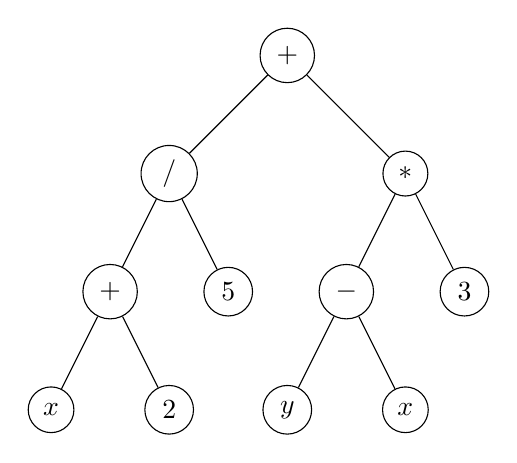
\begin{tikzpicture}[level 1/.style={sibling distance=30mm},level 2/.style={sibling distance=15mm}]
    \tikzstyle{every node}=[circle,draw]
    \node { $+$ }
        child {
            node { $/$ }
            child {
		node{ $+$ }
		child{ node{ $x$ } }
		child{ node{2} }
	    }
            child { node {5} }
        }
        child {
            node { $*$ }
            child { node { $-$ } 
		    child{ node{$y$} } 
		    child{ node{$x$} } 
		  }
            child { node {3} }
        }
    ;
\end{tikzpicture}\\[0.8cm]

At the leaves of the tree, we have input variables, ($x$ and $y$), and constant values (2, 5, and 3). Any 
such expression can be expressed this way. 

%how a parse tree can be defined by a string, given bla
Given any tree, we can take a traversal of the tree and make a string. Conversely, we can take a string, 
and use it to form a unique parse tree. For GEP, we call this a 'karva string'. The karva string of our 
previous example would be ``+/*+5-3x2yx''. Our algorithm for converting this into a parse tree is as follows:

\begin{enumerate}
 \item Read the first character, and make a root node. Add this node to the working list.
 \item If the worklist is empty, quit. 
 \item Read the next character. If it is a function, create a function node, and add it to the worklist. 
      Otherwise, create a ``free variable'' node, or ``constant node''.
 \item Get the first item in the worklist. Add the newly created node as a child of it.
 \item If the first item in the worklist has as many children as it should (all functions take a specific number of 
       inputs), then remove it from the worklist. 
 \item Go to 2.
\end{enumerate}

Applying this to our working example of ``+/*+5-3x2yx'', we would first create ``+'' as the root, then set it's 
children to be ``/'' and ``*'', adding each to the worklist. Since this means ``+'' has both of its 
two children, we remove it from the worklist. Continuing this process, we will eventually get the 
tree above. 

This algorithm makes a few specific assumptions. First, it assumes that all functions have a specific number of 
inputs. While in true mathematics, ``+'' may have many inputs, in this case we assume it has just 2. This still 
works, mathematically, as one of the children could be another ``+'', which has the same overall effect. 

The next assumption is that the original karva string will not leave us with items still in the worklist, but run out  
of characters. We can guarantee that this will always work, provided that the string meets certain conditions. 
We first choose a head length, $h$, where the head is first part of the string. The head can contain functions, 
constants, and free variables. The second part is the tail, which can contain only free variables and constants. 
If the head were to contain only functions, and each function was of the maximum number of arguments of any functions, 
then we would need to have enough elements in the tail to fill all the leaves in the tree. We can guarantee this, 
provided that the length of the tail, $t$ meets:

\[ t = h * (n_{max} - 1) + 1 \]

Where $n_{max}$ is the maximum number of arguments of any function available. When this is true, even in the worst 
case the karva string can be converted into a parse tree. 

\subsection{Genotypes and Phenotypes}
%how the GEA uses this to take a karva string, and make an expressed phenotype
The power of GEP comes from the separation between the simple string, and the complex parse trees that 
can be created from the strings. This mirrors the genotype-phenotype distinction we see in nature. Our 
karva string is our genotype: simple, non-active, easy to manipulate. Our parse tree is our phenotype: 
complex, active, hard to change, but powerful. Through this distinction, GEP gains its power.
By applying genetic operators (mutation, recombination) on the karva strings, and then applying 
fitness functions and selection on the expressed parse trees, we can mirror nature's evolution. 

\subsection{Random Numerical Constants}

Our parse tree example included some constant numbers. When evolving a parse tree with GEP, we want 
to have constants like this available. In order to facilitate this, we give each karva string a set 
of randomly generated numerical constants. These $k$ constants are numbered 0 to $k$, and can be 
used just like any free variable by our parse trees. What makes this especially powerful is GEPs 
ability to turn these random numbers into any value that is needed. 

For example, if three values generated are 0.5, 1.3 and 2.1, and we have the functions ``$+$'', ``$-$'', 
``$/$'' and ``$*$'', then we can combine any pair of these constants with any of the functions. 
Because some functions like ``$/$'' produce
different results based on the order of the inputs this 
can give us more than ${3 \choose 2} * 4$ values. 0.5 and 1.3 can become $0.5 + 1.3 = 1.8$, 
$0.5 - 1.3 = -0.8$, $0.5 * 1.3 = 0.65$ and $0.5 / 1.3 =  0.3846$. Reversing the minus or divide will 
produce even more results. 

Given 10 randomly generated values, this gives us more than 
${10 \choose 2} * 4 = 90$ different values, plus the original 10. So 10 random values becomes 100. 
We can do this again, using these 100 values, and get over 5000 potential values. Simply put, with 
10 random numerical constants, and just 4 functions, very good approximations can be generated 
of whatever value we need. 

\section{Artifical Neural Networks}

Artificial Neural Networks (ANN) are used as a tool for machine learning. They draw their inspiration 
from biological neural networks, but work quite differently.

%Description of a single perceptron/neuron
A single neuron in a classical ANN is called a perceptron. A single perceptron works as an on-off switch, 
triggered by a set of inputs, each multiplied by a weight. Given a set of inputs, $K$, to perceptron $p$, we can 
say that $p(K) = \sum\limits_{i=1}^{|K|} p_{w_i} * k_i $. The sum of the inputs multiplied by a specific 
weight for each input. If $p(K)$ is greater than some value $a$, the $p$ outputs $1$. Otherwise, it outputs $0$. 
Other types of ANNs may just always output the value given by the weighted sums, or a function of these outputs 
(for example, a sigmoid function will take any input, and return a value between -1 and 1, or 0 and 1).
These weights $p_w$ have to be set through training to ensure the correct output for different inputs. 

%description of a layer of neurons, description of a multi-layer perceptron, or ANN
A layer of perceptrons, $L$, is a list of perceptrons, taking the same inputs. Each will have its own set 
of weights, and give its own output based on the inputs. A set of layers, $M$, is known as a multi-layer 
perceptron. Each of the outputs of one layer is given as the inputs to the next layer. Given sufficient 
training, large enough layers, and enough hidden layers (layers between the input and output layers), very 
complex functions can be learned. Another name for a 
multi-layer perceptron is an Artificial Neural Network. 

ANNs can be applied to the problem of classification quite simply: in the output layer, we have one node 
for each potential class. Whichever output node activates, or whichever outputs the highest output value, 
is the class which this ANN has decided this input vector is associated with. We can train the network 
on a large set of input vectors with known classifications.

\section{Applying Gene Expression Programming to Artificial Neural Networks}

%explanation of main concept: replace the activator functions with expressed karva strings
To build an ANN using GEP, we will replace the activator function of each node of the network with a karva string, 
which is expressed as a parse tree when we want to get the output of the node. As before, each node has 
a return value for a number of input values, but rather than being a sum of the inputs multiplied by associated 
weights, we build custom functions, which can be much more complex. 

The entire ANN is then represented as a set of karva strings, which, when the output is desired, can be expressed 
as a series of parse trees. The typical ANN design, where each layer's output is the next layer's input, is used. 
Just like in classical ANNs for classification, we set the first set of inputs as input vector, each subsequent layer 
takes the previous layers outputs as its inputs, and the final output layer has one node for each potential class. 

%why this is so powerful (can do anything classic can do plus more, disregard useless data, find unusual relationships)
A classical ANN, with weights trained for each node, can be simulated nearly perfectly with a GEP ANN. The same function, 
adding each input and multiplying it by a weight, can be approximated by the parse tree, using the addition function, 
and the multiplication function. The weights can be approximated using the random numerical constants. Since GEP ANNs 
can form nearly the exact function of a classical ANN, and yet can still do more than they can, GEP ANNs can make even 
more powerful approximatations of whatever function they are trying to learn. 

\chapter{The GEP Framework}

\section{Framework description}
%High level view of the framework- it applies the algorithm
The GEP Framework is a framework for building classifiers using the GEP ANN design. It is given 
a Dataset to train against, a set of functions that can be used by the parse trees, mutators and crossover methods, 
as well as several other parameters like population size, and maximum number of generations. Running the 
evolver uses the genetic algorithm, and produces a GEP ANN for classification. 

%customizability of functions, fitness, selection
\section{Customizability}
The framework is designed with customizability in mind. Crossovers, mutators, functions, fitness methods and selection 
methods are all abstract interfaces. There are a small set of built-in implementations of all of these methods (for 
example, Addition, Subtraction, and other basic mathematical operators are all implemented as Functions). When the 
main graphical interface is run, a user is able to select which built-in types are desired to be used, as well as 
which custom-programmed classes the user wishes to use (which meet the appropriate framework interface). So if 
a user decides that a function should really be added to the evolver, all they must do is code it themselves, compile
it, and load it into the evolver's configuration with the graphical tool. 
As well, each custom class is allowed to have parameters which are used when it first initializes, so that it can 
be customized at runtime as needed, without changing code.

As well, to allow for inclusion of as much or as little complexity as desired, multiple crossover and mutation methods 
can be used in the framework, with each being given a weight value for how often they should be used. If two mutation methods 
exist, and the first has a weight 1, while the second has a weight 9, then the expected number of times the first is used 
is only 10\% of the time. 

%pipeline framework: add whatever you like
\section{Pipeline Framework}
Throughout the main genetic algorithm, a pipeline framework has been added to allow the user complete freedom in 
how the algorithm should be modified. Before and after each generation, before and after each run of the algorithm, 
and before and after the entire program, custom code can be executed. This is done through an additional interface, 
EvolverStateProcess, which can be implemented by the user in their own custom class, and loaded into the evolver's
configuration with the graphical tool. So if a user wishes to have the best member of the population saved to a file 
at the end of each generation, they write the code to do that functionality, then use the graphical tool to 
add that process to the 'end of generation' part of the pipeline. Parameters are also used by these EvolverStateProcesses
to allow for run-time customization. 

%examples of pipelined features, current and potential future
Currently, only basic pipeline features are implemented. Outputting the current configuration, outputting the 
score of the best member of the population, and recording the current score to a file. A process to increase the 
mutation rate based on how recently the best score has increased was also implemented as an example of more complex
functionality that can be added in this way. 

The potential for future processes is enormous. Graphical tools could be launched at the end of a run to output a 
pictorial representation of the best-found classifier. Efficient code in any language could be generated by a 
process based on the best-found classifier. The best-found of several runs of the algorithm could be saved, and 
combined into a more powerful system. The possibilities are endless.

\chapter{Experiments Conducted}

\section{Description of Tools}

In the experiments, a few specific mutators, crossovers and functions are used. Briefly, they will 
be described. 

\begin{itemize}
 \item \textbf{AddOneOnCorrect}: A fitness method where one point is added to the score for each instance of the training 
set correctly identified.
 \item \textbf{Basic Elitism}: A selection method in which just the top $x$ of the elements are kept, and the rest are removed.
 \item \textbf{RandomizeGene}: Mutation method where one gene, or one node in the network, is completely randomized.
 \item \textbf{RandomReplacement}: Mutation method where by one gene is selected, and one element in that gene is set to a 
random value from the list of possible values in that spot.
\item \textbf{Complexify}: Similar to RandomReplacement, except that only items in the head are picked, and the new 
value is always a function (thus, the node becomes more complex).
\item \textbf{OnePointPerLayer}: A crossover method. For each layer, a split point is chosen. 
All the genes before that point come from parent A, and all the rest of the genes from parent B. 
\item \textbf{CopyParentA}: A crossover method which simply makes a clone of one parent.
\end{itemize}

\section{Iris Plants Database}
%description of the data set, problem 
The Iris Plant Database is a classic dataset for machine learning and classification. It consists
of 3 types of iris plants, with 4 attributes. There are 50 instances of each class. One class is 
linearly separable from the others, but the remaining two are not linearly separable. This makes 
perfect classification very difficult.  

%Goal of the experiment
The goal of the experiment is to build a classifier with the highest classification level possible, 
using one subset of the training set for training, and the others for testing, to ensure overfitting 
does not occur. 

%Parameters of the experiment, configuration, etc

\begin{tabular}{| l | c |}
 \hline
 Title & Iris Plants Database \\
 \hline
 Number of Inputs & 4 \\
 Number of Classes & 3 \\
 Training Set Instances & 100 \\
 Testing Set Instances & 50 \\
 Number of Runs & 5 \\
 Number of Generations & 100 \\
 Population Size & 50 \\
 Functions & +,-,*,/,$\sqrt{}$,Sine \\
 Head Size & 5 \\
 Hidden Layers & 1: 10 nodes \\
 Fitness Process & AddOneOnCorrect \\
 Selection Process & Basic Elitism \\
 Mutators & RandomizeGene, RandomReplacement, Complexify \\
 Mutation Rate & 0.5 \\
 Crossovers & OnePointPerLayer, CopyParentA \\ 
 \hline
\end{tabular}


\section{Letter Image Recognition Data}
%description of the data set, problem
 The Letter Image Recongition Data is a dataset consisting of 20,000 instances of images of letters, in 
20 fonts, each distorted slightly. These images have been converted into 16 different attributes, each an 
integer value from 0 to 15. Typically, 16,000 of the instances are used for training, while 4,000 are used for
testing.

%goal of experiment
The goal of the experiment is to build a classifier with the highest classification level possible, 
using one subset of the training set for training, and the others for testing, to ensure overfitting 
does not occur. 

%parameters of the experiment, configuration, etc
\begin{tabular}{| l | c |}
 \hline
 Title & Letter Image Recognition Data \\
 \hline
 Number of Inputs & 16 \\
 Number of Classes & 26 \\
 Training Set Instances & 16000 \\
 Testing Set Instances & 4000 \\
 Number of Runs & 5 \\
 Number of Generations & 500 \\
 Population Size & 50 \\
 Functions & +,-,*,/,$\sqrt{}$,Sine \\
 Head Size & 5 \\
 Hidden Layers & 1: 60 nodes \\
 Fitness Process & AddOneOnCorrect \\
 Selection Process & Basic Elitism \\
 Mutators & RandomizeGene, RandomReplacement, Complexify \\
 Mutation Rate & 0.5 \\
 Crossovers & OnePointPerLayer, CopyParentA \\ 
 \hline
\end{tabular}

\section{Wisconsin Breast Cancer Database}
%description of the data set, problem


%goal of experiment


%parameters of the experiment, configuration, etc



\chapter{Results}




\chapter{Conclusion}


\chapter{References}

%FIND SOURCE:
%-Genetypes vs Phenotypes



\end{document}          
